% Figure 1 of docs/expert_companion.md: the columns, the winner's address and
% its selected cell. Build with tools/render_papers.py.
\documentclass[tikz,border=4pt]{standalone}
\usepackage{amsmath,amssymb}
\usetikzlibrary{arrows.meta,positioning,calc,decorations.pathreplacing}
\definecolor{one}{RGB}{226,232,240}
\definecolor{zero}{RGB}{40,40,40}
\definecolor{win}{RGB}{176,58,46}
\definecolor{addr}{RGB}{40,90,150}
\begin{document}
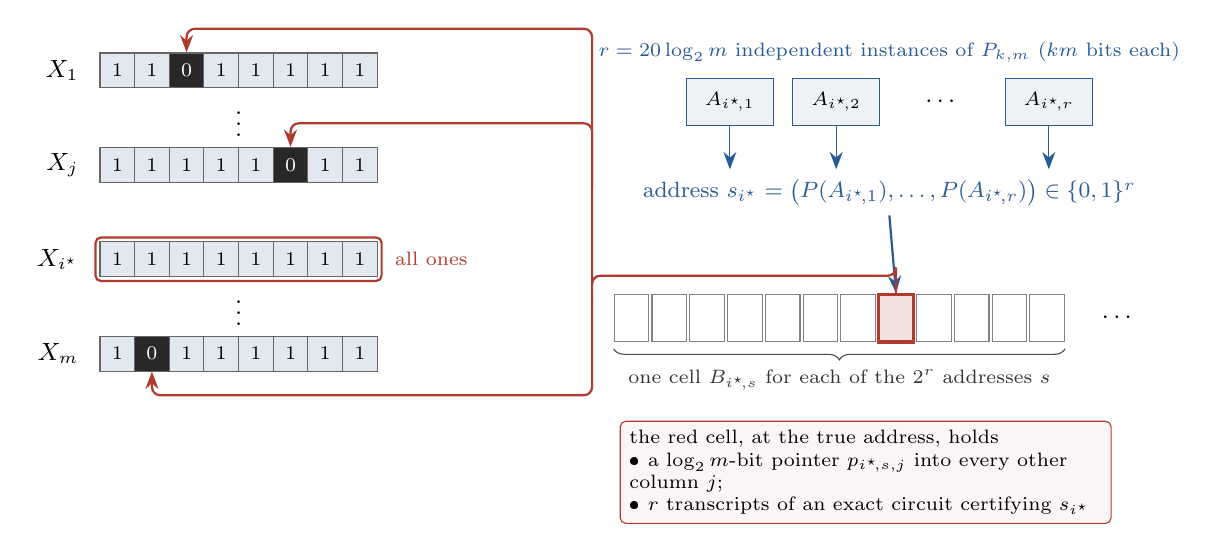
\begin{tikzpicture}[
  font=\small,
  bit/.style={draw=black!60, minimum width=4.4mm, minimum height=4.4mm,
              inner sep=0pt, font=\scriptsize},
  >={Stealth[length=2.2mm]}]
% ---- the strings X_j, drawn as rows of m = 8 bits -----------------------
\newcommand{\strip}[4]{% y, label, zero position (0 = none), name
  \node[anchor=east] at (-0.15,#1) {#2};
  \foreach \c in {1,...,8} {
    \ifnum\c=#3
      \node[bit, fill=zero, text=white] (#4\c) at (0.44*\c-0.22,#1) {0};
    \else
      \node[bit, fill=one] (#4\c) at (0.44*\c-0.22,#1) {1};
    \fi}}
\strip{3.0}{$X_1$}{3}{a}
\node at (1.76,2.42) {$\vdots$};
\strip{1.8}{$X_{j}$}{6}{b}
\strip{0.6}{$X_{i^\star}$}{0}{w}
\node at (1.76,0.02) {$\vdots$};
\strip{-0.6}{$X_m$}{2}{c}
\draw[win, thick, rounded corners=2pt] ($(w1.south west)+(-0.05,-0.05)$)
   rectangle ($(w8.north east)+(0.05,0.05)$);
\node[win, anchor=west, font=\scriptsize, align=left] at (3.62,0.6)
   {all ones};
% ---- the winner's address instances -------------------------------------
\begin{scope}[shift={(8.0,2.6)}]
  \foreach \h/\lab in {0/{A_{i^\star\!,1}},1/{A_{i^\star\!,2}},3/{A_{i^\star\!,r}}} {
    \node[draw=addr, fill=addr!8, minimum width=11mm, minimum height=6mm,
          font=\scriptsize] (A\h) at (1.35*\h,0) {$\lab$};}
  \node at (2*1.35,0) {$\cdots$};
  \node[font=\scriptsize, addr, anchor=south] at (1.35*1.5,0.38)
    {$r=20\log_2 m$ independent instances of $P_{k,m}$ ($km$ bits each)};
  \node[font=\footnotesize, addr] (s) at (1.35*1.5,-1.15)
    {address $s_{i^\star}=\bigl(P(A_{i^\star\!,1}),\dots,P(A_{i^\star\!,r})\bigr)\in\{0,1\}^r$};
  \foreach \h in {0,1,3} \draw[->, addr] (A\h.south) -- (A\h.south |- s.north);
\end{scope}
% ---- the cell array B_{i*,s}, s in {0,1}^r ------------------------------
\begin{scope}[shift={(6.75,-0.15)}]
  \foreach \c in {0,...,11} {
    \ifnum\c=7
      \node[draw=win, very thick, fill=win!15, minimum width=4.4mm,
            minimum height=6mm, inner sep=0pt] (cell\c) at (0.48*\c,0) {};
    \else
      \node[draw=black!50, fill=white, minimum width=4.4mm,
            minimum height=6mm, inner sep=0pt] (cell\c) at (0.48*\c,0) {};
    \fi}
  \node[anchor=west] at (5.85,0) {$\cdots$};
  \draw[decorate, decoration={brace, mirror, amplitude=4pt}, black!70]
    ($(cell0.south west)+(0,-0.08)$) -- ($(cell11.south east)+(0,-0.08)$)
    node[midway, below=4pt, font=\scriptsize, black!80]
    {one cell $B_{i^\star\!,s}$ for each of the $2^r$ addresses $s$};
\end{scope}
\draw[->, addr, thick] (s.south) -- (cell7.north);
% ---- what the selected cell holds ---------------------------------------
\node[draw=win, fill=win!5, rounded corners=2pt, align=left, font=\scriptsize,
      anchor=north west, text width=60mm] (content) at (6.6,-1.45)
  {the red cell, at the true address, holds\\
   \textbullet\ a $\log_2 m$-bit pointer $p_{i^\star\!,s,j}$ into every other column $j$;\\
   \textbullet\ $r$ transcripts of an exact circuit certifying $s_{i^\star}$};
% ---- outward pointers, routed along one vertical bus --------------------
\coordinate (bus) at (6.25,0);
\draw[win, thick, rounded corners=3pt, ->] (cell7.north) |- ($(cell7.north)+(0,0.22)$)
  -| ($(bus)+(0,0)$) |- ($(a3.north)+(0,0.3)$) -- (a3.north);
\draw[win, thick, rounded corners=3pt, ->] ($(bus)+(0,1.5)$) |- ($(b6.north)+(0,0.3)$) -- (b6.north);
\draw[win, thick, rounded corners=3pt, ->] ($(bus)+(0,0.07)$) |- ($(c2.south)+(0,-0.3)$) -- (c2.south);
\end{tikzpicture}
\end{document}
